\documentclass[1p]{elsarticle_modified}
%\bibliographystyle{elsarticle-num}

%\usepackage[colorlinks]{hyperref}
%\usepackage{abbrmath_seonhwa} %\Abb, \Ascr, \Acal ,\Abf, \Afrak
\usepackage{amsfonts}
\usepackage{amssymb}
\usepackage{amsmath}
\usepackage{amsthm}
\usepackage{scalefnt}
\usepackage{amsbsy}
\usepackage{kotex}
\usepackage{caption}
\usepackage{subfig}
\usepackage{color}
\usepackage{graphicx}
\usepackage{xcolor} %% white, black, red, green, blue, cyan, magenta, yellow
\usepackage{float}
\usepackage{setspace}
\usepackage{hyperref}

\usepackage{tikz}
\usetikzlibrary{arrows}

\usepackage{multirow}
\usepackage{array} % fixed length table
\usepackage{hhline}

%%%%%%%%%%%%%%%%%%%%%
\makeatletter
\renewcommand*\env@matrix[1][\arraystretch]{%
	\edef\arraystretch{#1}%
	\hskip -\arraycolsep
	\let\@ifnextchar\new@ifnextchar
	\array{*\c@MaxMatrixCols c}}
\makeatother %https://tex.stackexchange.com/questions/14071/how-can-i-increase-the-line-spacing-in-a-matrix
%%%%%%%%%%%%%%%

\usepackage[normalem]{ulem}

\newcommand{\msout}[1]{\ifmmode\text{\sout{\ensuremath{#1}}}\else\sout{#1}\fi}
%SOURCE: \msout is \stkout macro in https://tex.stackexchange.com/questions/20609/strikeout-in-math-mode

\newcommand{\cancel}[1]{
	\ifmmode
	{\color{red}\msout{#1}}
	\else
	{\color{red}\sout{#1}}
	\fi
}

\newcommand{\add}[1]{
	{\color{blue}\uwave{#1}}
}

\newcommand{\replace}[2]{
	\ifmmode
	{\color{red}\msout{#1}}{\color{blue}\uwave{#2}}
	\else
	{\color{red}\sout{#1}}{\color{blue}\uwave{#2}}
	\fi
}

\newcommand{\Sol}{\mathcal{S}} %segment
\newcommand{\D}{D} %diagram
\newcommand{\A}{\mathcal{A}} %arc


%%%%%%%%%%%%%%%%%%%%%%%%%%%%%5 test

\def\sl{\operatorname{\textup{SL}}(2,\Cbb)}
\def\psl{\operatorname{\textup{PSL}}(2,\Cbb)}
\def\quan{\mkern 1mu \triangleright \mkern 1mu}

\theoremstyle{definition}
\newtheorem{thm}{Theorem}[section]
\newtheorem{prop}[thm]{Proposition}
\newtheorem{lem}[thm]{Lemma}
\newtheorem{ques}[thm]{Question}
\newtheorem{cor}[thm]{Corollary}
\newtheorem{defn}[thm]{Definition}
\newtheorem{exam}[thm]{Example}
\newtheorem{rmk}[thm]{Remark}
\newtheorem{alg}[thm]{Algorithm}

\newcommand{\I}{\sqrt{-1}}
\begin{document}

%\begin{frontmatter}
%
%\title{Boundary parabolic representations of knots up to 8 crossings}
%
%%% Group authors per affiliation:
%\author{Yunhi Cho} 
%\address{Department of Mathematics, University of Seoul, Seoul, Korea}
%\ead{yhcho@uos.ac.kr}
%
%
%\author{Seonhwa Kim} %\fnref{s_kim}}
%\address{Center for Geometry and Physics, Institute for Basic Science, Pohang, 37673, Korea}
%\ead{ryeona17@ibs.re.kr}
%
%\author{Hyuk Kim}
%\address{Department of Mathematical Sciences, Seoul National University, Seoul 08826, Korea}
%\ead{hyukkim@snu.ac.kr}
%
%\author{Seokbeom Yoon}
%\address{Department of Mathematical Sciences, Seoul National University, Seoul, 08826,  Korea}
%\ead{sbyoon15@snu.ac.kr}
%
%\begin{abstract}
%We find all boundary parabolic representation of knots up to 8 crossings.
%
%\end{abstract}
%\begin{keyword}
%    \MSC[2010] 57M25 
%\end{keyword}
%
%\end{frontmatter}

%\linenumbers
%\tableofcontents
%
\newcommand\colored[1]{\textcolor{white}{\rule[-0.35ex]{0.8em}{1.4ex}}\kern-0.8em\color{red} #1}%
%\newcommand\colored[1]{\textcolor{white}{ #1}\kern-2.17ex	\textcolor{white}{ #1}\kern-1.81ex	\textcolor{white}{ #1}\kern-2.15ex\color{red}#1	}

{\Large $\underline{12a_{0826}~(K12a_{0826})}$}

\setlength{\tabcolsep}{10pt}
\renewcommand{\arraystretch}{1.6}
\vspace{1cm}\begin{tabular}{m{100pt}>{\centering\arraybackslash}m{274pt}}
\multirow{5}{120pt}{
	\centering
	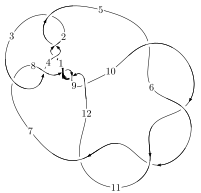
\includegraphics[width=112pt]{../../../GIT/diagram.site/Diagrams/png/1627_12a_0826.png}\\
\ \ \ A knot diagram\footnotemark}&
\allowdisplaybreaks
\textbf{Linearized knot diagam} \\
\cline{2-2}
 &
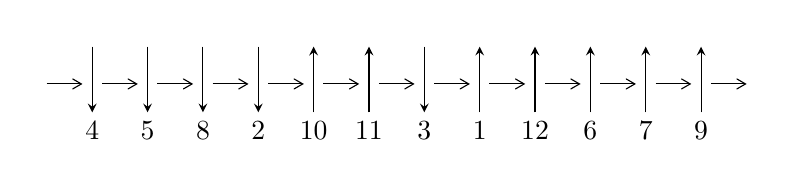
\begin{tikzpicture}[x=20pt, y=17pt]
	% nodes
	\node (C0) at (0, 0) {};
	\node (C1) at (1, 0) {};
	\node (C1U) at (1, +1) {};
	\node (C1D) at (1, -1) {4};

	\node (C2) at (2, 0) {};
	\node (C2U) at (2, +1) {};
	\node (C2D) at (2, -1) {5};

	\node (C3) at (3, 0) {};
	\node (C3U) at (3, +1) {};
	\node (C3D) at (3, -1) {8};

	\node (C4) at (4, 0) {};
	\node (C4U) at (4, +1) {};
	\node (C4D) at (4, -1) {2};

	\node (C5) at (5, 0) {};
	\node (C5U) at (5, +1) {};
	\node (C5D) at (5, -1) {10};

	\node (C6) at (6, 0) {};
	\node (C6U) at (6, +1) {};
	\node (C6D) at (6, -1) {11};

	\node (C7) at (7, 0) {};
	\node (C7U) at (7, +1) {};
	\node (C7D) at (7, -1) {3};

	\node (C8) at (8, 0) {};
	\node (C8U) at (8, +1) {};
	\node (C8D) at (8, -1) {1};

	\node (C9) at (9, 0) {};
	\node (C9U) at (9, +1) {};
	\node (C9D) at (9, -1) {12};

	\node (C10) at (10, 0) {};
	\node (C10U) at (10, +1) {};
	\node (C10D) at (10, -1) {6};

	\node (C11) at (11, 0) {};
	\node (C11U) at (11, +1) {};
	\node (C11D) at (11, -1) {7};

	\node (C12) at (12, 0) {};
	\node (C12U) at (12, +1) {};
	\node (C12D) at (12, -1) {9};
	\node (C13) at (13, 0) {};

	% arrows
	\draw[->,>={angle 60}]
	(C0) edge (C1) (C1) edge (C2) (C2) edge (C3) (C3) edge (C4) (C4) edge (C5) (C5) edge (C6) (C6) edge (C7) (C7) edge (C8) (C8) edge (C9) (C9) edge (C10) (C10) edge (C11) (C11) edge (C12) (C12) edge (C13) ;	\draw[->,>=stealth]
	(C1U) edge (C1D) (C2U) edge (C2D) (C3U) edge (C3D) (C4U) edge (C4D) (C5D) edge (C5U) (C6D) edge (C6U) (C7U) edge (C7D) (C8D) edge (C8U) (C9D) edge (C9U) (C10D) edge (C10U) (C11D) edge (C11U) (C12D) edge (C12U) ;
	\end{tikzpicture} \\
\hhline{~~} \\& 
\textbf{Solving Sequence} \\ \cline{2-2} 
 &
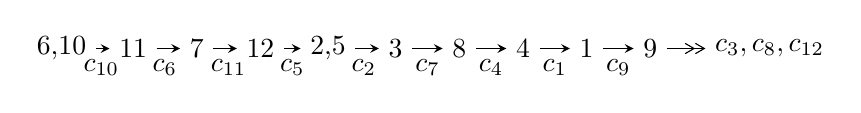
\begin{tikzpicture}[x=23pt, y=7pt]
	% node
	\node (A0) at (-1/8, 0) {6,10};
	\node (A1) at (1, 0) {11};
	\node (A2) at (2, 0) {7};
	\node (A3) at (3, 0) {12};
	\node (A4) at (65/16, 0) {2,5};
	\node (A5) at (41/8, 0) {3};
	\node (A6) at (49/8, 0) {8};
	\node (A7) at (57/8, 0) {4};
	\node (A8) at (65/8, 0) {1};
	\node (A9) at (73/8, 0) {9};
	\node (C1) at (1/2, -1) {$c_{10}$};
	\node (C2) at (3/2, -1) {$c_{6}$};
	\node (C3) at (5/2, -1) {$c_{11}$};
	\node (C4) at (7/2, -1) {$c_{5}$};
	\node (C5) at (37/8, -1) {$c_{2}$};
	\node (C6) at (45/8, -1) {$c_{7}$};
	\node (C7) at (53/8, -1) {$c_{4}$};
	\node (C8) at (61/8, -1) {$c_{1}$};
	\node (C9) at (69/8, -1) {$c_{9}$};
	\node (A10) at (11, 0) {$c_{3},c_{8},c_{12}$};

	% edge
	\draw[->,>=stealth]	
	(A0) edge (A1) (A1) edge (A2) (A2) edge (A3) (A3) edge (A4) (A4) edge (A5) (A5) edge (A6) (A6) edge (A7) (A7) edge (A8) (A8) edge (A9) ;
	\draw[->>,>={angle 60}]	
	(A9) edge (A10);
\end{tikzpicture} \\ 

\end{tabular} \\

\footnotetext{
The image of knot diagram is generated by the software ``\textbf{Draw programme}" developed by Andrew Bartholomew(\url{http://www.layer8.co.uk/maths/draw/index.htm\#Running-draw}), where we modified some parts for our purpose(\url{https://github.com/CATsTAILs/LinksPainter}).
}\phantom \\ \newline 
\centering \textbf{Ideals for irreducible components\footnotemark of $X_{\text{par}}$} 
 
\begin{align*}
I^u_{1}&=\langle 
u^{46}-24 u^{44}+\cdots+b-2 u,\;u^{49}- u^{48}+\cdots+a-3,\;u^{50}-2 u^{49}+\cdots-3 u+1\rangle \\
I^u_{2}&=\langle 
u^4-2 u^2+b,\;- u^5+3 u^3+a-2 u-1,\;u^6- u^5-3 u^4+2 u^3+2 u^2+u-1\rangle \\
\\
\end{align*}
\raggedright * 2 irreducible components of $\dim_{\mathbb{C}}=0$, with total 56 representations.\\
\footnotetext{All coefficients of polynomials are rational numbers. But the coefficients are sometimes approximated in decimal forms when there is not enough margin.}
\newpage
\renewcommand{\arraystretch}{1}
\centering \section*{I. $I^u_{1}= \langle u^{46}-24 u^{44}+\cdots+b-2 u,\;u^{49}- u^{48}+\cdots+a-3,\;u^{50}-2 u^{49}+\cdots-3 u+1 \rangle$}
\flushleft \textbf{(i) Arc colorings}\\
\begin{tabular}{m{7pt} m{180pt} m{7pt} m{180pt} }
\flushright $a_{6}=$&$\begin{pmatrix}0\\u\end{pmatrix}$ \\
\flushright $a_{10}=$&$\begin{pmatrix}1\\0\end{pmatrix}$ \\
\flushright $a_{11}=$&$\begin{pmatrix}1\\- u^2\end{pmatrix}$ \\
\flushright $a_{7}=$&$\begin{pmatrix}u\\- u^3+u\end{pmatrix}$ \\
\flushright $a_{12}=$&$\begin{pmatrix}- u^2+1\\u^4-2 u^2\end{pmatrix}$ \\
\flushright $a_{2}=$&$\begin{pmatrix}- u^{49}+u^{48}+\cdots+u+3\\- u^{46}+24 u^{44}+\cdots- u^2+2 u\end{pmatrix}$ \\
\flushright $a_{5}=$&$\begin{pmatrix}- u\\u\end{pmatrix}$ \\
\flushright $a_{3}=$&$\begin{pmatrix}u^{48}-25 u^{46}+\cdots+3 u+2\\- u^{49}+26 u^{47}+\cdots-8 u^2+1\end{pmatrix}$ \\
\flushright $a_{8}=$&$\begin{pmatrix}u^{14}-7 u^{12}+18 u^{10}-21 u^8+14 u^6-10 u^4+4 u^2-1\\- u^{16}+8 u^{14}-24 u^{12}+32 u^{10}-18 u^8+8 u^6-8 u^4\end{pmatrix}$ \\
\flushright $a_{4}=$&$\begin{pmatrix}-2 u^{49}+u^{48}+\cdots- u+3\\u^{49}-26 u^{47}+\cdots+5 u-1\end{pmatrix}$ \\
\flushright $a_{1}=$&$\begin{pmatrix}- u^{10}+5 u^8-8 u^6+5 u^4-3 u^2+1\\u^{12}-6 u^{10}+12 u^8-8 u^6+u^4-2 u^2\end{pmatrix}$ \\
\flushright $a_{9}=$&$\begin{pmatrix}- u^6+3 u^4-2 u^2+1\\u^8-4 u^6+4 u^4\end{pmatrix}$\\&\end{tabular}
\flushleft \textbf{(ii) Obstruction class $= -1$}\\~\\
\flushleft \textbf{(iii) Cusp Shapes $= 4 u^{49}-7 u^{48}+\cdots-34 u-6$}\\~\\
\newpage\renewcommand{\arraystretch}{1}
\flushleft \textbf{(iv) u-Polynomials at the component}\newline \\
\begin{tabular}{m{50pt}|m{274pt}}
Crossings & \hspace{64pt}u-Polynomials at each crossing \\
\hline $$\begin{aligned}c_{1},c_{2},c_{4}\end{aligned}$$&$\begin{aligned}
&u^{50}-7 u^{49}+\cdots+2 u-1
\end{aligned}$\\
\hline $$\begin{aligned}c_{3},c_{7}\end{aligned}$$&$\begin{aligned}
&u^{50}- u^{49}+\cdots+224 u^2-64
\end{aligned}$\\
\hline $$\begin{aligned}c_{5},c_{6},c_{10}\\c_{11}\end{aligned}$$&$\begin{aligned}
&u^{50}+2 u^{49}+\cdots+3 u+1
\end{aligned}$\\
\hline $$\begin{aligned}c_{8},c_{9},c_{12}\end{aligned}$$&$\begin{aligned}
&u^{50}+6 u^{49}+\cdots+45 u-9
\end{aligned}$\\
\hline
\end{tabular}\\~\\
\newpage\renewcommand{\arraystretch}{1}
\flushleft \textbf{(v) Riley Polynomials at the component}\newline \\
\begin{tabular}{m{50pt}|m{274pt}}
Crossings & \hspace{64pt}Riley Polynomials at each crossing \\
\hline $$\begin{aligned}c_{1},c_{2},c_{4}\end{aligned}$$&$\begin{aligned}
&y^{50}-53 y^{49}+\cdots+24 y+1
\end{aligned}$\\
\hline $$\begin{aligned}c_{3},c_{7}\end{aligned}$$&$\begin{aligned}
&y^{50}-39 y^{49}+\cdots-28672 y+4096
\end{aligned}$\\
\hline $$\begin{aligned}c_{5},c_{6},c_{10}\\c_{11}\end{aligned}$$&$\begin{aligned}
&y^{50}-54 y^{49}+\cdots-23 y+1
\end{aligned}$\\
\hline $$\begin{aligned}c_{8},c_{9},c_{12}\end{aligned}$$&$\begin{aligned}
&y^{50}+54 y^{49}+\cdots-2871 y+81
\end{aligned}$\\
\hline
\end{tabular}\\~\\
\newpage\flushleft \textbf{(vi) Complex Volumes and Cusp Shapes}
$$\begin{array}{c|c|c}  
\text{Solutions to }I^u_{1}& \I (\text{vol} + \sqrt{-1}CS) & \text{Cusp shape}\\
 \hline 
\begin{aligned}
u &= -0.553117 + 0.664163 I \\
a &= \phantom{-}1.18281 - 1.02165 I \\
b &= -0.27217 + 2.65461 I\end{aligned}
 & -15.1392 - 9.4868 I & -4.47770 + 6.36607 I \\ \hline\begin{aligned}
u &= -0.553117 - 0.664163 I \\
a &= \phantom{-}1.18281 + 1.02165 I \\
b &= -0.27217 - 2.65461 I\end{aligned}
 & -15.1392 + 9.4868 I & -4.47770 - 6.36607 I \\ \hline\begin{aligned}
u &= -0.521122 + 0.653186 I \\
a &= -0.360363 - 0.132250 I \\
b &= \phantom{-}0.744618 - 1.077000 I\end{aligned}
 & -7.98509 - 5.12361 I & -2.94810 + 5.86362 I \\ \hline\begin{aligned}
u &= -0.521122 - 0.653186 I \\
a &= -0.360363 + 0.132250 I \\
b &= \phantom{-}0.744618 + 1.077000 I\end{aligned}
 & -7.98509 + 5.12361 I & -2.94810 - 5.86362 I \\ \hline\begin{aligned}
u &= -0.832663\phantom{ +0.000000I} \\
a &= \phantom{-}1.37585\phantom{ +0.000000I} \\
b &= \phantom{-}0.379950\phantom{ +0.000000I}\end{aligned}
 & -4.23580\phantom{ +0.000000I} & \phantom{-}0.843030\phantom{ +0.000000I} \\ \hline\begin{aligned}
u &= \phantom{-}0.505395 + 0.660908 I \\
a &= \phantom{-}1.86551 + 1.12155 I \\
b &= -0.76904 - 2.58054 I\end{aligned}
 & -10.25710 + 2.22642 I & -3.92809 - 3.01901 I \\ \hline\begin{aligned}
u &= \phantom{-}0.505395 - 0.660908 I \\
a &= \phantom{-}1.86551 - 1.12155 I \\
b &= -0.76904 + 2.58054 I\end{aligned}
 & -10.25710 - 2.22642 I & -3.92809 + 3.01901 I \\ \hline\begin{aligned}
u &= -0.460008 + 0.686028 I \\
a &= \phantom{-}2.07694 - 0.50744 I \\
b &= -0.71544 + 1.92454 I\end{aligned}
 & -15.4170 + 4.9513 I & -5.18278 - 0.57560 I \\ \hline\begin{aligned}
u &= -0.460008 - 0.686028 I \\
a &= \phantom{-}2.07694 + 0.50744 I \\
b &= -0.71544 - 1.92454 I\end{aligned}
 & -15.4170 - 4.9513 I & -5.18278 + 0.57560 I \\ \hline\begin{aligned}
u &= -0.487371 + 0.659703 I \\
a &= -0.906971 + 0.645379 I \\
b &= -0.393135 - 0.627704 I\end{aligned}
 & -8.08531 + 0.69745 I & -3.35798 + 0.23540 I\\
 \hline 
 \end{array}$$\newpage$$\begin{array}{c|c|c}  
\text{Solutions to }I^u_{1}& \I (\text{vol} + \sqrt{-1}CS) & \text{Cusp shape}\\
 \hline 
\begin{aligned}
u &= -0.487371 - 0.659703 I \\
a &= -0.906971 - 0.645379 I \\
b &= -0.393135 + 0.627704 I\end{aligned}
 & -8.08531 - 0.69745 I & -3.35798 - 0.23540 I \\ \hline\begin{aligned}
u &= \phantom{-}0.660442 + 0.437938 I \\
a &= -1.175670 - 0.632150 I \\
b &= -0.27825 + 1.82886 I\end{aligned}
 & -6.65255 + 5.49617 I & -1.92374 - 6.88073 I \\ \hline\begin{aligned}
u &= \phantom{-}0.660442 - 0.437938 I \\
a &= -1.175670 + 0.632150 I \\
b &= -0.27825 - 1.82886 I\end{aligned}
 & -6.65255 - 5.49617 I & -1.92374 + 6.88073 I \\ \hline\begin{aligned}
u &= \phantom{-}0.494871 + 0.598464 I \\
a &= -0.642916 - 0.366018 I \\
b &= \phantom{-}0.316810 + 0.829305 I\end{aligned}
 & -3.61220 + 2.04087 I & \phantom{-}3.66627 - 3.62580 I \\ \hline\begin{aligned}
u &= \phantom{-}0.494871 - 0.598464 I \\
a &= -0.642916 + 0.366018 I \\
b &= \phantom{-}0.316810 - 0.829305 I\end{aligned}
 & -3.61220 - 2.04087 I & \phantom{-}3.66627 + 3.62580 I \\ \hline\begin{aligned}
u &= -1.34345\phantom{ +0.000000I} \\
a &= \phantom{-}2.34922\phantom{ +0.000000I} \\
b &= -1.18992\phantom{ +0.000000I}\end{aligned}
 & -3.73496\phantom{ +0.000000I} & \phantom{-0.000000 } 0 \\ \hline\begin{aligned}
u &= \phantom{-}0.539188 + 0.357182 I \\
a &= -0.060078 - 0.229300 I \\
b &= \phantom{-}0.065780 - 0.818765 I\end{aligned}
 & -0.53394 + 3.00224 I & \phantom{-}1.62141 - 9.45825 I \\ \hline\begin{aligned}
u &= \phantom{-}0.539188 - 0.357182 I \\
a &= -0.060078 + 0.229300 I \\
b &= \phantom{-}0.065780 + 0.818765 I\end{aligned}
 & -0.53394 - 3.00224 I & \phantom{-}1.62141 + 9.45825 I \\ \hline\begin{aligned}
u &= \phantom{-}0.197556 + 0.567801 I \\
a &= -1.33311 + 0.94398 I \\
b &= \phantom{-}0.34749 + 1.38106 I\end{aligned}
 & -8.06992 - 2.05324 I & -6.14708 + 0.44806 I \\ \hline\begin{aligned}
u &= \phantom{-}0.197556 - 0.567801 I \\
a &= -1.33311 - 0.94398 I \\
b &= \phantom{-}0.34749 - 1.38106 I\end{aligned}
 & -8.06992 + 2.05324 I & -6.14708 - 0.44806 I\\
 \hline 
 \end{array}$$\newpage$$\begin{array}{c|c|c}  
\text{Solutions to }I^u_{1}& \I (\text{vol} + \sqrt{-1}CS) & \text{Cusp shape}\\
 \hline 
\begin{aligned}
u &= -0.432575 + 0.376085 I \\
a &= -1.94487 + 0.34224 I \\
b &= \phantom{-}0.40285 - 1.84963 I\end{aligned}
 & -2.72128 - 1.34903 I & -0.70979 + 4.63030 I \\ \hline\begin{aligned}
u &= -0.432575 - 0.376085 I \\
a &= -1.94487 - 0.34224 I \\
b &= \phantom{-}0.40285 + 1.84963 I\end{aligned}
 & -2.72128 + 1.34903 I & -0.70979 - 4.63030 I \\ \hline\begin{aligned}
u &= -0.523312 + 0.099839 I \\
a &= \phantom{-}0.392896 + 0.049847 I \\
b &= -0.497458 + 0.355216 I\end{aligned}
 & \phantom{-}0.918277 - 0.180115 I & \phantom{-}10.59554 + 1.05153 I \\ \hline\begin{aligned}
u &= -0.523312 - 0.099839 I \\
a &= \phantom{-}0.392896 - 0.049847 I \\
b &= -0.497458 - 0.355216 I\end{aligned}
 & \phantom{-}0.918277 + 0.180115 I & \phantom{-}10.59554 - 1.05153 I \\ \hline\begin{aligned}
u &= -1.48986 + 0.04819 I \\
a &= -0.213305 - 0.758850 I \\
b &= -0.383824 + 1.018250 I\end{aligned}
 & \phantom{-}4.60096 - 0.59150 I & \phantom{-0.000000 } 0 \\ \hline\begin{aligned}
u &= -1.48986 - 0.04819 I \\
a &= -0.213305 + 0.758850 I \\
b &= -0.383824 - 1.018250 I\end{aligned}
 & \phantom{-}4.60096 + 0.59150 I & \phantom{-0.000000 } 0 \\ \hline\begin{aligned}
u &= \phantom{-}1.47972 + 0.21886 I \\
a &= -2.61247 - 0.77557 I \\
b &= \phantom{-}1.52280 + 0.76083 I\end{aligned}
 & -9.13237 - 1.69237 I & \phantom{-0.000000 } 0 \\ \hline\begin{aligned}
u &= \phantom{-}1.47972 - 0.21886 I \\
a &= -2.61247 + 0.77557 I \\
b &= \phantom{-}1.52280 - 0.76083 I\end{aligned}
 & -9.13237 + 1.69237 I & \phantom{-0.000000 } 0 \\ \hline\begin{aligned}
u &= \phantom{-}1.50421 + 0.08278 I \\
a &= \phantom{-}2.26526 + 2.33731 I \\
b &= -1.43825 - 2.50580 I\end{aligned}
 & \phantom{-}3.72115 + 2.85609 I & \phantom{-0.000000 } 0 \\ \hline\begin{aligned}
u &= \phantom{-}1.50421 - 0.08278 I \\
a &= \phantom{-}2.26526 - 2.33731 I \\
b &= -1.43825 + 2.50580 I\end{aligned}
 & \phantom{-}3.72115 - 2.85609 I & \phantom{-0.000000 } 0\\
 \hline 
 \end{array}$$\newpage$$\begin{array}{c|c|c}  
\text{Solutions to }I^u_{1}& \I (\text{vol} + \sqrt{-1}CS) & \text{Cusp shape}\\
 \hline 
\begin{aligned}
u &= \phantom{-}1.50288 + 0.20473 I \\
a &= \phantom{-}0.247045 + 0.583522 I \\
b &= \phantom{-}0.259330 - 0.087519 I\end{aligned}
 & -1.58696 + 2.41508 I & \phantom{-0.000000 } 0 \\ \hline\begin{aligned}
u &= \phantom{-}1.50288 - 0.20473 I \\
a &= \phantom{-}0.247045 - 0.583522 I \\
b &= \phantom{-}0.259330 + 0.087519 I\end{aligned}
 & -1.58696 - 2.41508 I & \phantom{-0.000000 } 0 \\ \hline\begin{aligned}
u &= -1.51678 + 0.17371 I \\
a &= \phantom{-}1.27783 - 0.63401 I \\
b &= -0.991957 + 0.734002 I\end{aligned}
 & \phantom{-}3.01331 - 4.79464 I & \phantom{-0.000000 } 0 \\ \hline\begin{aligned}
u &= -1.51678 - 0.17371 I \\
a &= \phantom{-}1.27783 + 0.63401 I \\
b &= -0.991957 - 0.734002 I\end{aligned}
 & \phantom{-}3.01331 + 4.79464 I & \phantom{-0.000000 } 0 \\ \hline\begin{aligned}
u &= -1.51343 + 0.20796 I \\
a &= -3.33763 + 1.93254 I \\
b &= \phantom{-}2.35728 - 2.09370 I\end{aligned}
 & -3.64700 - 5.36770 I & \phantom{-0.000000 } 0 \\ \hline\begin{aligned}
u &= -1.51343 - 0.20796 I \\
a &= -3.33763 - 1.93254 I \\
b &= \phantom{-}2.35728 + 2.09370 I\end{aligned}
 & -3.64700 + 5.36770 I & \phantom{-0.000000 } 0 \\ \hline\begin{aligned}
u &= \phantom{-}1.53588 + 0.02926 I \\
a &= -1.104940 - 0.849103 I \\
b &= \phantom{-}1.04875 + 1.10169 I\end{aligned}
 & \phantom{-}7.88396 + 0.66037 I & \phantom{-0.000000 } 0 \\ \hline\begin{aligned}
u &= \phantom{-}1.53588 - 0.02926 I \\
a &= -1.104940 + 0.849103 I \\
b &= \phantom{-}1.04875 - 1.10169 I\end{aligned}
 & \phantom{-}7.88396 - 0.66037 I & \phantom{-0.000000 } 0 \\ \hline\begin{aligned}
u &= -1.53405 + 0.08867 I \\
a &= -0.256516 + 1.388440 I \\
b &= \phantom{-}0.10053 - 1.82714 I\end{aligned}
 & \phantom{-}6.40849 - 4.54154 I & \phantom{-0.000000 } 0 \\ \hline\begin{aligned}
u &= -1.53405 - 0.08867 I \\
a &= -0.256516 - 1.388440 I \\
b &= \phantom{-}0.10053 + 1.82714 I\end{aligned}
 & \phantom{-}6.40849 + 4.54154 I & \phantom{-0.000000 } 0\\
 \hline 
 \end{array}$$\newpage$$\begin{array}{c|c|c}  
\text{Solutions to }I^u_{1}& \I (\text{vol} + \sqrt{-1}CS) & \text{Cusp shape}\\
 \hline 
\begin{aligned}
u &= \phantom{-}1.52299 + 0.20532 I \\
a &= \phantom{-}1.60846 + 0.80229 I \\
b &= -1.32719 - 1.42793 I\end{aligned}
 & -1.27126 + 8.23471 I & \phantom{-0.000000 } 0 \\ \hline\begin{aligned}
u &= \phantom{-}1.52299 - 0.20532 I \\
a &= \phantom{-}1.60846 - 0.80229 I \\
b &= -1.32719 + 1.42793 I\end{aligned}
 & -1.27126 - 8.23471 I & \phantom{-0.000000 } 0 \\ \hline\begin{aligned}
u &= \phantom{-}0.270980 + 0.357042 I \\
a &= \phantom{-}1.336840 - 0.453135 I \\
b &= \phantom{-}0.0735636 - 0.0211419 I\end{aligned}
 & -1.313390 - 0.394009 I & -4.59693 - 0.11426 I \\ \hline\begin{aligned}
u &= \phantom{-}0.270980 - 0.357042 I \\
a &= \phantom{-}1.336840 + 0.453135 I \\
b &= \phantom{-}0.0735636 + 0.0211419 I\end{aligned}
 & -1.313390 + 0.394009 I & -4.59693 + 0.11426 I \\ \hline\begin{aligned}
u &= \phantom{-}1.53896 + 0.21280 I \\
a &= -2.44076 - 2.71196 I \\
b &= \phantom{-}1.46316 + 3.05025 I\end{aligned}
 & -8.2472 + 12.6896 I & \phantom{-0.000000 } 0 \\ \hline\begin{aligned}
u &= \phantom{-}1.53896 - 0.21280 I \\
a &= -2.44076 + 2.71196 I \\
b &= \phantom{-}1.46316 - 3.05025 I\end{aligned}
 & -8.2472 - 12.6896 I & \phantom{-0.000000 } 0 \\ \hline\begin{aligned}
u &= -1.57081 + 0.11496 I \\
a &= \phantom{-}0.54586 - 2.32961 I \\
b &= \phantom{-}0.35877 + 2.51364 I\end{aligned}
 & \phantom{-}0.85171 - 7.47143 I & \phantom{-0.000000 } 0 \\ \hline\begin{aligned}
u &= -1.57081 - 0.11496 I \\
a &= \phantom{-}0.54586 + 2.32961 I \\
b &= \phantom{-}0.35877 - 2.51364 I\end{aligned}
 & \phantom{-}0.85171 + 7.47143 I & \phantom{-0.000000 } 0 \\ \hline\begin{aligned}
u &= \phantom{-}1.59062\phantom{ +0.000000I} \\
a &= \phantom{-}0.786115\phantom{ +0.000000I} \\
b &= -1.65951\phantom{ +0.000000I}\end{aligned}
 & \phantom{-}3.85485\phantom{ +0.000000I} & \phantom{-0.000000 } 0 \\ \hline\begin{aligned}
u &= \phantom{-}0.284196\phantom{ +0.000000I} \\
a &= \phantom{-}2.66910\phantom{ +0.000000I} \\
b &= \phantom{-}0.479450\phantom{ +0.000000I}\end{aligned}
 & -1.25005\phantom{ +0.000000I} & -12.8860\phantom{ +0.000000I}\\
 \hline 
 \end{array}$$\newpage\newpage\renewcommand{\arraystretch}{1}
\centering \section*{II. $I^u_{2}= \langle u^4-2 u^2+b,\;- u^5+3 u^3+a-2 u-1,\;u^6- u^5-3 u^4+2 u^3+2 u^2+u-1 \rangle$}
\flushleft \textbf{(i) Arc colorings}\\
\begin{tabular}{m{7pt} m{180pt} m{7pt} m{180pt} }
\flushright $a_{6}=$&$\begin{pmatrix}0\\u\end{pmatrix}$ \\
\flushright $a_{10}=$&$\begin{pmatrix}1\\0\end{pmatrix}$ \\
\flushright $a_{11}=$&$\begin{pmatrix}1\\- u^2\end{pmatrix}$ \\
\flushright $a_{7}=$&$\begin{pmatrix}u\\- u^3+u\end{pmatrix}$ \\
\flushright $a_{12}=$&$\begin{pmatrix}- u^2+1\\u^4-2 u^2\end{pmatrix}$ \\
\flushright $a_{2}=$&$\begin{pmatrix}u^5-3 u^3+2 u+1\\- u^4+2 u^2\end{pmatrix}$ \\
\flushright $a_{5}=$&$\begin{pmatrix}- u\\u\end{pmatrix}$ \\
\flushright $a_{3}=$&$\begin{pmatrix}u^5-3 u^3+u+1\\- u^4+2 u^2+u\end{pmatrix}$ \\
\flushright $a_{8}=$&$\begin{pmatrix}u\\- u^3+u\end{pmatrix}$ \\
\flushright $a_{4}=$&$\begin{pmatrix}u^5-3 u^3+u+1\\- u^4+2 u^2+u\end{pmatrix}$ \\
\flushright $a_{1}=$&$\begin{pmatrix}u\\- u\end{pmatrix}$ \\
\flushright $a_{9}=$&$\begin{pmatrix}- u^5+2 u^3+u\\u^5-3 u^3+u\end{pmatrix}$\\&\end{tabular}
\flushleft \textbf{(ii) Obstruction class $= 1$}\\~\\
\flushleft \textbf{(iii) Cusp Shapes $= 3 u^5- u^4-14 u^3+u^2+14 u+6$}\\~\\
\newpage\renewcommand{\arraystretch}{1}
\flushleft \textbf{(iv) u-Polynomials at the component}\newline \\
\begin{tabular}{m{50pt}|m{274pt}}
Crossings & \hspace{64pt}u-Polynomials at each crossing \\
\hline $$\begin{aligned}c_{1},c_{2}\end{aligned}$$&$\begin{aligned}
&(u-1)^6
\end{aligned}$\\
\hline $$\begin{aligned}c_{3},c_{7}\end{aligned}$$&$\begin{aligned}
&u^6
\end{aligned}$\\
\hline $$\begin{aligned}c_{4}\end{aligned}$$&$\begin{aligned}
&(u+1)^6
\end{aligned}$\\
\hline $$\begin{aligned}c_{5},c_{6}\end{aligned}$$&$\begin{aligned}
&u^6+u^5-3 u^4-2 u^3+2 u^2- u-1
\end{aligned}$\\
\hline $$\begin{aligned}c_{8},c_{9}\end{aligned}$$&$\begin{aligned}
&u^6- u^5+3 u^4-2 u^3+2 u^2- u-1
\end{aligned}$\\
\hline $$\begin{aligned}c_{10},c_{11}\end{aligned}$$&$\begin{aligned}
&u^6- u^5-3 u^4+2 u^3+2 u^2+u-1
\end{aligned}$\\
\hline $$\begin{aligned}c_{12}\end{aligned}$$&$\begin{aligned}
&u^6+u^5+3 u^4+2 u^3+2 u^2+u-1
\end{aligned}$\\
\hline
\end{tabular}\\~\\
\newpage\renewcommand{\arraystretch}{1}
\flushleft \textbf{(v) Riley Polynomials at the component}\newline \\
\begin{tabular}{m{50pt}|m{274pt}}
Crossings & \hspace{64pt}Riley Polynomials at each crossing \\
\hline $$\begin{aligned}c_{1},c_{2},c_{4}\end{aligned}$$&$\begin{aligned}
&(y-1)^6
\end{aligned}$\\
\hline $$\begin{aligned}c_{3},c_{7}\end{aligned}$$&$\begin{aligned}
&y^6
\end{aligned}$\\
\hline $$\begin{aligned}c_{5},c_{6},c_{10}\\c_{11}\end{aligned}$$&$\begin{aligned}
&y^6-7 y^5+17 y^4-16 y^3+6 y^2-5 y+1
\end{aligned}$\\
\hline $$\begin{aligned}c_{8},c_{9},c_{12}\end{aligned}$$&$\begin{aligned}
&y^6+5 y^5+9 y^4+4 y^3-6 y^2-5 y+1
\end{aligned}$\\
\hline
\end{tabular}\\~\\
\newpage\flushleft \textbf{(vi) Complex Volumes and Cusp Shapes}
$$\begin{array}{c|c|c}  
\text{Solutions to }I^u_{2}& \I (\text{vol} + \sqrt{-1}CS) & \text{Cusp shape}\\
 \hline 
\begin{aligned}
u &= -0.493180 + 0.575288 I \\
a &= -0.997760 + 0.232521 I \\
b &= \phantom{-}0.138835 - 1.234450 I\end{aligned}
 & -4.60518 - 1.97241 I & -5.56070 + 3.48596 I \\ \hline\begin{aligned}
u &= -0.493180 - 0.575288 I \\
a &= -0.997760 - 0.232521 I \\
b &= \phantom{-}0.138835 + 1.234450 I\end{aligned}
 & -4.60518 + 1.97241 I & -5.56070 - 3.48596 I \\ \hline\begin{aligned}
u &= \phantom{-}0.483672\phantom{ +0.000000I} \\
a &= \phantom{-}1.65437\phantom{ +0.000000I} \\
b &= \phantom{-}0.413150\phantom{ +0.000000I}\end{aligned}
 & -0.906083\phantom{ +0.000000I} & \phantom{-}11.4460\phantom{ +0.000000I} \\ \hline\begin{aligned}
u &= \phantom{-}1.52087 + 0.16310 I \\
a &= \phantom{-}1.05885 + 1.20667 I \\
b &= -0.408802 - 1.276380 I\end{aligned}
 & \phantom{-}2.05064 + 4.59213 I & -1.33400 - 2.48468 I \\ \hline\begin{aligned}
u &= \phantom{-}1.52087 - 0.16310 I \\
a &= \phantom{-}1.05885 - 1.20667 I \\
b &= -0.408802 + 1.276380 I\end{aligned}
 & \phantom{-}2.05064 - 4.59213 I & -1.33400 + 2.48468 I \\ \hline\begin{aligned}
u &= -1.53904\phantom{ +0.000000I} \\
a &= \phantom{-}0.223460\phantom{ +0.000000I} \\
b &= -0.873214\phantom{ +0.000000I}\end{aligned}
 & \phantom{-}6.01515\phantom{ +0.000000I} & \phantom{-}6.34350\phantom{ +0.000000I}\\
 \hline 
 \end{array}$$\newpage
\newpage\renewcommand{\arraystretch}{1}
\centering \section*{ III. u-Polynomials}
\begin{tabular}{m{50pt}|m{274pt}}
Crossings & \hspace{64pt}u-Polynomials at each crossing \\
\hline $$\begin{aligned}c_{1},c_{2}\end{aligned}$$&$\begin{aligned}
&((u-1)^6)(u^{50}-7 u^{49}+\cdots+2 u-1)
\end{aligned}$\\
\hline $$\begin{aligned}c_{3},c_{7}\end{aligned}$$&$\begin{aligned}
&u^6(u^{50}- u^{49}+\cdots+224 u^2-64)
\end{aligned}$\\
\hline $$\begin{aligned}c_{4}\end{aligned}$$&$\begin{aligned}
&((u+1)^6)(u^{50}-7 u^{49}+\cdots+2 u-1)
\end{aligned}$\\
\hline $$\begin{aligned}c_{5},c_{6}\end{aligned}$$&$\begin{aligned}
&(u^6+u^5-3 u^4-2 u^3+2 u^2- u-1)(u^{50}+2 u^{49}+\cdots+3 u+1)
\end{aligned}$\\
\hline $$\begin{aligned}c_{8},c_{9}\end{aligned}$$&$\begin{aligned}
&(u^6- u^5+3 u^4-2 u^3+2 u^2- u-1)(u^{50}+6 u^{49}+\cdots+45 u-9)
\end{aligned}$\\
\hline $$\begin{aligned}c_{10},c_{11}\end{aligned}$$&$\begin{aligned}
&(u^6- u^5-3 u^4+2 u^3+2 u^2+u-1)(u^{50}+2 u^{49}+\cdots+3 u+1)
\end{aligned}$\\
\hline $$\begin{aligned}c_{12}\end{aligned}$$&$\begin{aligned}
&(u^6+u^5+3 u^4+2 u^3+2 u^2+u-1)(u^{50}+6 u^{49}+\cdots+45 u-9)
\end{aligned}$\\
\hline
\end{tabular}\newpage\renewcommand{\arraystretch}{1}
\centering \section*{ IV. Riley Polynomials}
\begin{tabular}{m{50pt}|m{274pt}}
Crossings & \hspace{64pt}Riley Polynomials at each crossing \\
\hline $$\begin{aligned}c_{1},c_{2},c_{4}\end{aligned}$$&$\begin{aligned}
&((y-1)^6)(y^{50}-53 y^{49}+\cdots+24 y+1)
\end{aligned}$\\
\hline $$\begin{aligned}c_{3},c_{7}\end{aligned}$$&$\begin{aligned}
&y^6(y^{50}-39 y^{49}+\cdots-28672 y+4096)
\end{aligned}$\\
\hline $$\begin{aligned}c_{5},c_{6},c_{10}\\c_{11}\end{aligned}$$&$\begin{aligned}
&(y^6-7 y^5+\cdots-5 y+1)(y^{50}-54 y^{49}+\cdots-23 y+1)
\end{aligned}$\\
\hline $$\begin{aligned}c_{8},c_{9},c_{12}\end{aligned}$$&$\begin{aligned}
&(y^6+5 y^5+\cdots-5 y+1)(y^{50}+54 y^{49}+\cdots-2871 y+81)
\end{aligned}$\\
\hline
\end{tabular}
\vskip 2pc
\end{document}